\chapter{The Polygonal JCT: Part II}\label{chapter:JordanVerification2}
In this chapter, we shall discuss the second half of the Jordan Curve Theorem for polygons based on the axioms of Hilbert's ordered geometry, and our verification of this theorem in HOL~Light. In this half of the theorem, we must prove that a simple polygon separates its plane into at most two regions. As discussed when we gave the formalisation of this theorem in Chapter~\ref{chapter:JordanFormalisation}, it amounts to proving that given three points in the plane and not on the polygon, at least two of them are connected by a polygonal path.

This is effectively a maze navigation problem, and it has a pleasing visual interpretation. Unlike the ``crossings'' of the last chapter, the basic concepts we appeal to can be realised faithfully in the low-level details of the formalisation, rather than being obscured by case-analyses and edge cases. 

In discussing our verification, we will cover the same basic ground as we did in the last chapter. In \S\ref{sec:SketchProofJordan2}, we shall give an overview of the proof structure, effectively amounting to a sketch proof of the theorem. In \S\ref{sec:Jordan2Formulation}, we will look more closely at some of the basic ideas behind the sketch proof, and formalise them in higher-order logic. Then, in \S\ref{sec:Jordan2Lemmas}, we shall cover the key lemmas that support our basic formalised concepts. As in the last chapter, we shall divide these lemmas between those which introduce points in a geometrical configuration, and those which allow us to infer properties of the resulting configurations. 

In the rest of the chapter, we shall look in more detail at how the lemmas are applied to recover all the details of the sketch proof. We provide a few readable extracts of what we hope are interesting proofs, demonstrating how faithfully we can formalise the intuitive synthetic arguments.

\section{Sketch Proof}\label{sec:SketchProofJordan2}
The basic intuition behind the proof is similar to the ones presented by Veblen~\cite{Veblenphd} and Feigl~\cite{FeiglJordan}. We follow Veblen's proof the most closely. Contary to Guggenheimer's~\cite{GuggenheimerJordanCurve} claim that Veblen's proof only holds for convex polygons, we believe it is basically correct. That said, our verification is based on a more thorough analysis than presented by Veblen.

We are required to show that, given three points in the plane and not on a polygon, at least two of them are connected by a polygonal path. Let us reinterpret this and understand the three points as three players trying to navigate a polygonal maze. Each edge of the polygon can then be thought of as a maze \emph{wall}.

Our basic goal is to get the three players ``next to'' the same wall. Then we just need to find a path between whichever of the two players are on the same side of that wall. We will find that the difficulty here lies in getting the players through potentially very tight corridors, and around difficult corners. We must show how to obtain paths for the players without recourse to notions such as comparable directions, parallel lines or distances. This will rule out common approaches to the theorem, such as the one given by Tverberg~\cite{TverbergJordan}. In Tverberg's proof, we just need to consider a sufficiently small region around the walls of the maze (an ``offset curve'' ), which we know to be path-connected. Without notions of distance, this description is out of scope of Hilbert's ordered geometry.

One way to formulate the idea that the players are ``next to'' the same wall of the maze is to assert that all three have line-of-sight to that wall. This metaphor does not appear explicitly in Veblen or Feigl's proof, but it can be read into both, and we found it extremely helpful in providing an intuitive grasp of the formalisation.

In Figure~\ref{fig:SketchProofJordan2}, we show players $Red$, $Black$ and $Blue$ starting at various points of a maze. Players $Red$ and $Black$ are inside the maze, while $Blue$ is on the outside. Here, we depict the paths they follow as they traverse the maze so that they have line-of-sight to the wall $P_iP_{i+1}$. Since $Red$ and $Black$ are on the same side of $P_iP_{i+1}$, we can connect them by a polygonal path.

\begin{figure}
  \centering\includegraphics[scale=0.75]{jordanVerification2/SketchProof}
  \caption{Navigating a Maze}
  \label{fig:SketchProofJordan2}
\end{figure}

The paths we have drawn through the maze are potential witnesses to the paths we consider in our verification. In fact, we can take the line-extension axiom 
\begin{equation}
  \tag{\ref{eq:g22}}
  \vdash A \neq B \implies \exists C. \between{A}{B}{C}
\end{equation}
and suppose that the witness $C$ in the conclusion is always chosen so that $B$ is half-way between $A$ and $C$. In this case, the paths sketched in Figure~\ref{fig:SketchProofJordan2} are precisely those that we witness in our formal verification.

\section{Formulation and Formalisation}\label{sec:Jordan2Formulation}
Compared to the last chapter, where we introduce the complex idea of a crossing, the basic ideas needed in the proof for this chapter are relatively straightforward. Firstly, given a simple polygon $Ps$, we will say that a point $X$ has line-of-sight to be a point $X'$ if there is no point of $Ps$ which lies strictly between $X$ and $X'$. In diagrams such as Figure~\ref{fig:SketchProofJordan2}, we shall always depict the point $X$ as an eye pointed at $X'$, with a dashed line indicating the line-of-sight. We shall also say that when the point $X'$ lies between vertices $P_i$ and $P_{i+1}$ of $Ps$, then the point $X$ has line-of-sight to the \emph{wall} $P_iP_{i+1}$. The situation is formalised as
\begin{displaymath}
  \begin{aligned}
    &\neg\code{on\_polypath}\ Ps\ X \wedge \between{P_i}{X'}{P_{i+1}}\\
    &\wedge \neg\exists Z. \between{X}{Z}{X'} \wedge \code{on\_polypath}\ Ps\ Z
  \end{aligned}
\end{displaymath}

Our formalised proof breaks down into three parts. Firstly, we must show how every point not on a simple polygon has a line-of-sight to some wall of the maze. Next, we must show how, if a point $X$ has line-of-sight to a wall $P_iP_{i+1}$, then there is a polygonal path to a point $Y$ which has line-of-sight to the next wall $P_{i+1}P_{i+2}$. As such, for any wall and any point $X$, there is a polygonal path from $X$ to another point which has line-of-sight to that wall. Finally, we must show that if two players have line-of-sight to the same wall, and lie on the same side of that wall, then there is a polygonal path between them.
We shall describe the informal proofs and verifications of each part in \S\ref{sec:NavigationVerification}.

First, we consider the crucial supporting lemmas.

\section{Obtaining Lines-of-Sight}\label{sec:Jordan2Lemmas}
We have two key theorems: a ray-casting theorem which obtains a new line-of-sight, and a theorem dubbed ``squeeze'' which handles narrow cracks in corridors. In proving the ``squeeze'' theorem, we shall need recourse to many of our earlier theorems about triangles and their interiors, and a new theorem about a triangle containing another triangle.

\subsection{Ray-casting}\label{sec:RayCasting}
Our ray-casting theorem gives us a line-of-sight to a polygonal path, aimed in an arbitrary direction towards that path. To achieve this, we must find the first point of intersection that the ray makes with the polygonal path. Ray-casting is actually needed in the first half of the Polygonal Jordan Curve Theorem (see \S\ref{sec:FinalProofJordan1}), but it makes more sense to explain it in this section where we are  self-consciously using metaphors from computer graphics.

Ray-casting appears in a weakened form in Veblen's proof, but there he only considers casting a ray which does not intersect any \emph{vertex} of the polygonal path. This can be generalised by considering a few additional cases, after which we have a much more useful theorem.

This ray-casting theorem is the only major theorem since Hilbert's \ref{eq:seven} which relies almost exclusively on linear reasoning. We also found it proved to be particularly tricky. As with our proof of Theorem~\ref{eq:IH3} in the last chapter, our linear reasoning tactic came through as a powerful tool for dealing with these problems, but first it has to be fed the right starting hypotheses. The trouble we had in the ray-casting proof was deciding which hypotheses were needed. 

Finding the necessary hypotheses often ended up being a matter of trial and error, but fortunately, the linear reasoning tactic is based on a \emph{decision procedure}. When there were not enough facts available, it would promptly terminate and announce that the goal was not solvable. We could then go back through the problem and try to identify additional facts to feed the tactic and then retry. 

In a few places, we found that what we were missing was a case-split. Sometimes, this reflected two different linear reasoning problems, which meant providing two subproofs. But sometimes we got lucky. If the case split led to a single linear reasoning problem, we could let our incidence-discoverer handle the case-analyses automatically using its internal representation of proof trees.

The basic proof applies structural induction on the vertex list, and reduces the problem to that of ray-casting to a single edge. The basic case-analyses are shown in Figure~\ref{fig:RayCast}. We cast rays from the points $A$, $B$ and $C$ to the polygonal path $P_1P_2\ldots P_5$. The salient differences between the three lines-of-sight are as follows: point $A$ has line-of-sight to an endpoint of an edge, but the edge itself is not on the line-of-sight. Point $B$ has line-of-sight to an endpoint of an edge, and the edge itself \emph{is} on the line-of-sight. Finally, point $C$ has line-of-sight to the interior of an edge $P_2P_3$. 

\begin{figure}
\centering\includegraphics[scale=0.75]{jordanVerification2/RayCast}
\caption{Ray-casting}
\label{fig:RayCast}
\end{figure}

We now give the formalisation of the theorem. From a point $X$, we fire a ray to an arbitrary point $P$ on the polygonal path, and then obtain a point $Y$ to which $X$ has line-of-sight. Though it does not prove necessary in our proofs, we provide some extra information about the point $Y$, namely that it is either strictly between $X$ and $P$, or else we already had line-of-sight to $P$. 

\begin{equation}\label{eq:RayCast}
% |- !Ps X Y.
%          ~on_polyseg Ps X /\ on_polyseg Ps P
%          ==> (?Z. on_polyseg Ps Z /\
%                   (between X Z Y \/ Y = Z) /\
%                   ~(?R. between X R Z /\ on_polyseg Ps R))
  \begin{aligned}
    \vdash&\neg\code{on\_polypath}\ Ps\ X \wedge \code{on\_polypath}\ Ps\ P\\
    &\implies \exists Y. \code{on\_polypath}\ Ps\ Y \wedge \between{X}{Y}{P} \vee X = P)\\
    &\qquad\qquad \wedge \neg(\exists Q. \between{X}{Q}{Y} \wedge \code{on\_polypath}\ Ps\ R).
  \end{aligned}
\end{equation}

Note the first conjunct in the hypothesis of this theorem. We can only cast rays to a polygonal path if we are not on that path. This should clarify a point made in \S\ref{sec:FinalProofJordan1} of the last chapter. There, we said that the final part of the proof showing that there are at least two regions of a simple polygon is based on ray-casting \emph{from} some point $X$ on that polygon. In particular, we are ray-casting to the \emph{rest} of the polygon, and thus, if we are to ray-cast, we need to assume that the rest of the polygon does not have a self-intersection at $X$. This we guarantee based on the fact that the polygon is assumed to be \emph{simple}.

\subsection{Squeeze}\label{sec:Squeeze}
The most powerful theorem in our development towards the Jordan Curve Theorem is one we dubbed \emph{squeeze}, since the intuition is that it allows us to find segments which squeeze through arbitrarily narrow gaps of a maze. Again, what counts as a narrow gap in the abstract world of ordered geometry is only determined by the three-place \emph{betweenness} relation. Our ability to navigate these gaps must therefore reduce to just the basic axioms governing this relation. We can get some idea of the challenge by realising that, on some interpretations, these gaps are \emph{infinitesimally} narrow. Hilbert's axioms are independent of Archimedes' axiom.

Abstractly, the theorem tells us that if we have a polygonal path $[A,B,C]$ which is not intersected by the polygonal path $Ps$, then there is a point $A'$ between $A$ and $C$ such that $Ps$ intersects $AC$ in at most one place. We can understand this in the context of finding diagonals of simple polygons, as is described in Figure~\S\ref{sec:FindingDiagonal}. In fact, this was the original motivation for \emph{squeeze}, and we have retained its conclusion in a form which is still fit for this purpose. It thus remains an important component of a verification for our sketch proof in \S\ref{sec:JordanCurveFirstProof}. In \S\ref{sec:SqueezeEye}, we will show how to interpret it in terms of lines-of-sight.
\begin{equation}\label{eq:Squeeze}
  \begin{aligned}
      % "!P start goal 'a polyseg.
      % ~(?a. on_line P a /\ on_line start a /\ on_line goal a)
      % /\ on_plane P 'a /\ on_plane start 'a /\ on_plane goal 'a
      % /\ (!X. MEM X polyseg ==> on_plane X 'a)
      % /\ ~on_polyseg polyseg P
      % /\ (!X. between P X start ==> ~on_polyseg polyseg X)
      % /\ (!X. between P X goal ==> ~on_polyseg polyseg X)
      % ==> ?s. between P s start
      %         /\ !X. in_triangle (P,s,goal) X ==> ~on_polyseg polyseg X"
    \vdash&\neg\code{on\_polypath}\ path\ B\\
    &\wedge \neg(\exists X. \between{A}{X}{B} \wedge \code{on\_polypath}\ path\ X)\\
    &\wedge \neg(\exists X. \between{B}{X}{C} \wedge \code{on\_polypath}\ path\ X)\\
    &\implies \exists A'. \between{A}{A'}{B} \wedge \neg\exists X. \code{in\_triangle}\ (A',B,C) \wedge \code{on\_polypath}\ path\ X.
  \end{aligned}
\end{equation}

\begin{figure}
\centering\includegraphics[scale=0.75]{jordanVerification2/SqueezeDiagonal}
\caption{Squeezing a Diagonal}
\label{fig:SqueezeDiagonal}
\end{figure}

In Figure~\ref{fig:SqueezeDiagonal}, we show how \emph{squeeze} would be used to find a diagonal of the polygon $P_1P_2\ldots P_{11}$. Here, we have set $A = P_1$, $B = P_{11}$, and $C = P_{10}$, while we set $path$ to be the rest of the polygon $P_1P_2P_3\ldots P_{10}$. 

There are two points to note about our conclusion. Firstly, we make a stronger claim than merely declaring the existence of a diagonal. We say instead that the polygonal path does not lie in the interior of $\triangle A'BC$, which means that any point between $A'$ and $B$ yields a diagonal with the point $C$. Secondly, even though the witness $A'$ is defined in our proof to be such that a vertex $P_8$ of $Ps$ lies on $A'B$, we have not provided this additional information in the conclusion. Such information would be needed if our diagonal is to split the polygon into two simpler polygons, as needed for our first sketch proof in \S\ref{sec:JordanCurveFirstProof}. We \emph{have} verified this theorem with the additional information provided. However, for the purposes of the current proof, we present only the version with the simpler conclusion.

The mention of triangle interiors in the conclusion reflects the way the proof recursively verifies that $A'C$ really is a diagonal. Conceptually, the proof starts with the triangle $ABC$, and finds the first vertex in $Ps$ which lies inside this triangle. In the case shown, this would be the vertex $P_3$. We then draw a line through $P_{10}$ and $P_3$ to the point $A_3$, and continue the argument with this new triangle. Eventually, we will be left with a triangle whose interior contains no point of $Ps$. In a sense, the triangle $ABC$ has been ``squeezed'' by $Ps$ into the triangle $A'BC$.

Unhappily, proving that $\triangle A'BC$ contains no point of $Ps$ has us boiled down in case-splits similar to those needed to analyse triangle \emph{crossings} in the last chapter (\S\ref{sec:CrossingVerification}). Rather than go into the details of these, we shall focus on the more illuminating proof that $A'BC$ contains no \emph{vertex} of $Ps$. This only boils down to two more lemmas for triangle interiors.

\subsubsection{Another ``Inner Pasch'' Rule}
Our first supporting theorem is a point introduction rule which allows us to find the intersection points $A_3$, $A_4$, $A_6$ and $A'$ in Figure~\ref{fig:SqueezeDiagonal}. This theorem is similar in spirit to the Pasch axioms (\ref{eq:InnerPasch}, \ref{eq:OuterPasch}) and its variant for triangle interiors \eqref{eq:tricut1}. It has a very succinct formalisation, but a non-trivial verification:
\begin{equation}\label{eq:TriCut3}
\vdash\code{in\_triangle}\ (A,B,C)\ P \implies \exists X. \between{B}{X}{C} \wedge \between{A}{P}{X}.
\end{equation}

The proof is the most interesting of these point introduction rule proofs. Unlike the proof of Theorem~\ref{eq:TriCut3}, we find ourselves back employing Pasch's axiom \eqref{eq:g24} rather than exploiting our theorems of half-planes. First, we use \ref{eq:three} to find a point $X$ on $AB$. Next, we apply \eqref{eq:g24} to the triangle $ABC$ and the line $PX$. This gives us a point $Y$ which is either between $B$ and $C$ or between $A$ and $C$. Here is one of the rare times where both cases are possible. Normally, we would be able refute one of the cases based on incidence reasoning. Here, we need two subproofs.

\begin{figure}
\centering\includegraphics[scale=0.75]{jordanVerification2/TriCut3}
\caption{Drawing a line from a Vertex to the Opposite Side}
\label{fig:TriCut3}
\end{figure}

If $Y$ lies between $B$ and $C$ as in case (a) of Figure~\ref{fig:TriCut3}, then we apply \eqref{eq:g24} to the triangle $BXY$ and the line $AP$ to find a point between $B$ and $Y$. This point is then between $B$ and $C$ (via linear reasoning on $B$, $C$, $Y$ and $Z$). Furthermore, $P$ is between $A$ and $Z$ by~\eqref{eq:inTriangle2}.

In case (b) of Figure~\ref{fig:TriCut3}, we find that $P$ is now an interior point according to Veblen's definition, in virtue of the points $X$ and $Y$. Here, we apply \eqref{eq:g24} to the triangle $CXY$ and the line $AP$ to find a point $P'$ on $CX$. By the same axiom applied to $\triangle BCX$ and the line $AP'$, we find the desired point $Z$ on $BC$.

\subsubsection{Subtriangles}
In our proof of Theorem~\ref{eq:Squeeze}, we consider a sequence of triangles $\triangle ABC$, $\triangle A_3BC$, $\triangle A_4BC$, $\triangle A_6BC$ and $\triangle A'BC$. Each of these is intended to exclude one vertex of $Ps$ from its interior. By the time we reach the last triangle, we can conclude that all vertices of $Ps$ will lie in the exterior. This conclusion assumes a transitivity property, which is given by our second lemma. It shows that the ordering of $A$, $A_3$, $A_4$, $A_6$ and $A'$ along the segment $AB$ yields a sequence of triangles with \emph{nested} interiors. 

The proof, given in Figure~\ref{fig:SubTriangle}, is extremely short and readable, making use of a number of lemmas we have previously considered, including Theorem~\ref{eq:TriCut3} from the last subsection. With this theorem, we can put a point $Q$ on the line $A'C$, where we know it must be interior to $\triangle ABC$ on the basis of Theorem~\ref{eq:inTriangle1}. It then follows by Theorem~\ref{eq:inTriangle2} that $P$ must also be interior.

\begin{figure}
\centering\includegraphics[scale=0.75]{jordanVerification2/SubTriangle}
\caption{Any interior point $P$ of $\triangle ABC$ is an interior point of $\triangle AB'C$.}
\end{figure}

\begin{boxedfigure}
\small
\begin{align*}
&\code{theorem }\code{in\_triangle}\ (A,A',C)\ P \wedge \between{A}{A'}{B} 
                  \implies \code{in\_triangle}\ (A,B,C)\ P\\
&\code{assume}\ \code{in\_triangle}\ (A,A',C)\ P \wedge \between{A}{A'}{B} & 0 \\
&\code{so consider}\ Q\ \code{such that}\ \between{A'}{Q}{C} \wedge \between{A}{P}{Q} & 1\\
&\code{obviously}\ \code{(by\_ncols}\ \circ\ \code{add\_in\_triangle}\ \circ\ \code{conjuncts})\\
&\qquad \code{hence}\ \code{in\_triangle}\ (A,B,C)\ Q\ \code{by}\ \eqref{eq:triSyms},\eqref{eq:inTriangle1},\eqref{eq:g21}\ \code{from}\ 0\\
&\code{qed from}\ 1\ \code{by}\ \eqref{eq:onTriangleDef},\eqref{eq:inTriangle2}
\end{align*}
\caption{``Subtriangles''}
\label{fig:SubTriangle}
\end{boxedfigure}

\subsection{Obtaining lines-of-sight via Squeeze}\label{sec:SqueezeEye}
As we suggested earlier, Theorem~\ref{eq:Squeeze} is quite powerful, and allows us to do more than obtain diagonals. In this section, we will show two applications of the theorem in terms of lines-of-sight, both of which we shall need for the core proofs of this chapter. 

\subsubsection{Moving to a new line-of-sight}\label{sec:MoveToNew}
\begin{figure}
\centering\includegraphics[scale=0.75]{jordanVerification2/Squeeze1}
\caption{Obtaining line-of-sight to $C$}
\label{fig:Squeeze1}
\end{figure}

Consider Figure~\ref{fig:Squeeze1}. Here, we are not interested in diagonals, so we have slightly modified and relabelled the diagram from Figure~\ref{fig:SqueezeDiagonal}. Now we want to interpret the point $A$ is our player's starting location, with line-of-sight to a point $B$ on the wall $P_{11}P_{12}$ of a simple polygon. The goal is to obtain line-of-sight to a given point $C$ on that same wall.

The idea is that if the player proceeds far enough down their initial line-of-sight, we can easily rotate them to the new line-of-sight. We do this by applying Theorem~\ref{eq:Squeeze} and taking $path$ to be the fragment of the polygon $P_{12}P_1P_2\ldots P_{11}$. Let us think about how to fulfill the hypotheses. We are basically being asked to rule out the possibility that the polygonal path $[A,B,C]$ is not intersected by this fragment, save for possible intersections at $A$ and at $C$. 

Well, we know that the segment $AB$ does not lie on the path $P_{11}P_1P_2\ldots P_{11}$, because $AB$ is supposed to be a line-of-sight. We also know that $BC$ does not intersect $P_{11}P_{12}$, because we are assuming \emph{simple} polygons: the polygon should not self-intersect the edge $P_{11}P_{12}$, and this edge contains $BC$. We will still the possibility that $P_{11}P_1P_2\ldots P_{11}$ intersects the lone point $C$, since as we shall see in \S\ref{sec:ConcaveMove}, we will sometimes need to obtain line-of-sight to a vertex, and thus set $C=P_{11}$.

Applying Theorem~\ref{eq:Squeeze} is not quite enough. We now have a point $A'$ which \emph{almost} has line-of-sight to $C$. But that point $A'$ was originally intended to give us diagonals of polygons intersecting at least one vertex, and that vertex ($P_8$) is still in our way. We can fix this using \ref{eq:three}, obtaining a point $A''$ and a segment $A''C$ which lies properly in the triangle $A'BC$, and, as per the conclusion of \eqref{eq:Squeeze}, a segment which is a line-of-sight to the point $C$. We capture all of this in a corollary:
\begin{equation}\label{eq:Squeeze2}
  \begin{aligned}
  % "!P start goal 'a polyseg.
  %     ~(?a. on_line P a /\ on_line start a /\ on_line goal a)
  %     /\ on_plane P 'a /\ on_plane start 'a /\ on_plane goal 'a
  %     /\ (!X. MEM X polyseg ==> on_plane X 'a)
  %     /\ ~on_polyseg polyseg P
  %     /\ (!X. between P X start ==> ~on_polyseg polyseg X)
  %     /\ (!X. between P X goal ==> ~on_polyseg polyseg X)
  %     ==> (?s. between P s start
  %              /\ !X. between s X goal  ==> ~on_polyseg polyseg X)"
\vdash    &\neg\code{on\_polypath}\ path\ B\\
    &\wedge \neg(\exists X. \between{A}{X}{B} \wedge \code{on\_polypath}\ path\ X)\\
    &\wedge \neg(\exists X. \between{B}{X}{C} \wedge \code{on\_polypath}\ path\ X)\\
    &\implies \exists A'. \between{A}{A'}{B} \wedge \neg\exists X. \between{A'}{X}{C} \wedge \code{on\_polypath}\ path\ X.
  \end{aligned}
\end{equation}

Now because $AB$ was a line-of-sight, we know that $AA''$ is part of a polygonal path which does not intersect $P_1P_2\ldots P_{11}P_{12}P_{1}$. What we have exploited here is the fact that we can always move along our lines-of-sight without intersecting the polygon. The use of squeeze in this section is therefore telling us how to build up paths through a maze, by getting the player to move far enough along their line-of-sight that they will be able to see a point further down the current wall. 

The next use of squeeze will be just as critical for our proof.

\subsubsection{Rotating to a new line-of-sight}\label{sec:RotateToNew}
\begin{figure}
\centering\includegraphics[scale=0.75]{jordanVerification2/Squeeze2}
\caption{Obtaining line-of-sight to the interior of $AB$}
\label{fig:Squeeze2}
\end{figure}
In Figure~\ref{fig:Squeeze2}, we have again modified and relabelled the diagram. The idea here is that our player is situated at a point $C$ and initially has line-of-sight to the \emph{vertex} $B$. The problem with this scenario is that, in our proof, we are more concerned about having lines-of-sight to points on a polygon which are \emph{not} vertices (for a start, this forces the player off the line of the wall).  So we want our player to rotate their line-of-sight slightly. 

Therefore, we apply Theorem~\ref{eq:Squeeze} by reversing the order of $A$, $B$ and $C$. The polygon fragment we are concerned with here is again $P_{12}P_1P_2\ldots P_{11}$, and as before, we have to be sure that the hypotheses of Theorem~\ref{eq:Squeeze} have been met. That is, we must show that the polygonal path $[A,B,C]$ is not intersected by the fragment $P_{12}P_1P_2\ldots P_{11}$. 

Again, we know that $AB$ is not intersected by the fragment, because we assume that the polygon is simple and so does not have such self-intersections, and we know that $BC$ is not intersected by the fragment because $BC$ is assumed to be a line-of-sight. This means we have met the hypotheses. We now obtain the point $A'$ as shown, and as before, we use \ref{eq:three} to obtain a point $A''$ between $B$ and $A'$. This player will now have line-of-sight to a non-vertex point of the segment $AB$.

The reader may have noticed that we have not mentioned the segment $BP_{12}$ shown in the diagram. In fact, this segment could prove a problem. If it were chosen to lie on the other side of $BC$, then it might intersect the segment $A''C$, and if this happens, then $A''C$ will not count as a line-of-sight. Fortunately, we shall be able to rule out this circumstance when we come to apply this version of Axiom~\ref{eq:Squeeze2}. We shall always be assuming that, when we rotate our line-of-sight, the point $P_{12}$ will be known to be on the opposite side of $BC$ as the point $P_{11}$, as shown.

To summarise, we can say that the first use of Theorem~\ref{eq:Squeeze2} allows us to reduce the \emph{distance} to the point $B$ sufficiently and thus obtain a new line-of-sight, while this second use of squeeze is telling us that we can reduce the \emph{angle} $ABC$ sufficiently. What the theorem gives us is the ability to reduce distances and angles even without a general theory for comparing them, and without any sort of arithmetic for them. We ``squeeze'' our distances and angles by working exclusively with a weak order relation and properties of incidence.

\section{Wall-to-Wall}\label{sec:NavigationVerification}
Since a simple polygon is just a list of adjacent edges, we can navigate every single wall just by moving between one wall and the next in the adjacency list. In Section~\ref{sec:Jordan2Formulation}, we explained that the movement from a wall $P_{i}P_{i+1}$ to a wall $P_{i+1}P_{i+2}$ amounts to showing three things: (1) that there is a point $X$ with line-of-sight to $P_{i}P_{i+1}$; (2) that there is a point $Y$ with line-of-sight to $P_{i+1}P_{i+2}$; and (3), that there is a polygonal path between $X$ and $Y$.

Now when inside a convex polygon, this matter is completely trivial. Indeed, \emph{every} interior point of a convex polygon has line-of-sight to \emph{every} wall, as in Figure~\ref{fig:ConvexEasy}. The salient fact to notice is that, in a convex polygon, interior points are on the same side of every wall as every other vertex. 

\begin{figure}
\centering\includegraphics[scale=0.75]{jordanVerification2/ConvexEasy}
\caption{Wall-to-wall in a convex polygon}
\label{fig:ConvexEasy}
\end{figure}

Generalising this, we can say that two walls $P_{i}P_{i+1}$ and $P_{i+1}P_{i+2}$ appear ``locally convex'' from the perspective of a point $P$ if the point $P$ is on the same side of $P_{i}P_{i+1}$ as $P_{i+2}$ (and equivalently, on the same side of $P_{i+1}P_{i+2}$ as $P_{i}$). Otherwise, we can say that the walls appear ``locally concave''. These provide our two cases for how we navigate the walls of a simple polygon.

\subsection{Locally Convex Walls}\label{sec:ConcaveMove}
In this subsection, we shall deal with the case of locally convex walls. Here, we shall assume we have a polygon $P_1P_2P_3\ldots P_n$, and we shall assume that we are moving from wall $P_1P_2$ to wall $P_2P_3$ (we can use the polygon rotations described in \S\ref{sec:PolygonRotation} to consider the other pairs of walls).

\begin{figure}
\centering\includegraphics[scale=0.75]{jordanVerification2/Convex1}
\caption{Wall-to-wall in a locally convex polygon}
\label{fig:Convex1}
\end{figure}

In Figure~\ref{fig:Convex1}, we start at a point $X$ which has line-of-sight to $P_1P_2$. Our goal is to reach a point $Y$ with line-of-sight to $P_2P_3$. We start by moving towards $P_1P_2$ by applying Theorem~\ref{eq:Squeeze2} as described in \S\ref{sec:MoveToNew}, seeking a line-of-sight with the vertex~$P_2$. 

Applying squeeze in this way is usually a tricky business, because there are a number of hypotheses which must be fulfilled and it is not always immediately clear how. We typically started procedurally. First, we would assert our goal without any justification:

\fbox{\begin{minipage}{\linewidth}\setlength\abovedisplayskip{0cm}
\begin{multline*}
    % &\neg\code{on\_polypath}\ path\ B\\
    % &\wedge \neg(\exists X. \between{A}{X}{B} \wedge \code{on\_polypath}\ path\ X)\\
    % &\wedge \neg(\exists X. \between{B}{X}{C} \wedge \code{on\_polypath}\ path\ X)\\
    % &\implies \exists A'. \between{A}{A'}{B} \wedge \neg\exists X. \between{A'}{X}{C} \wedge \code{on\_polypath}\ path\ X.
\small
\code{consider}\ Y\ \code{such that}\ \between{X}{Y}{X'}\\ \wedge \neg\exists Z. \between{Y}{Z}{P_2} \wedge \code{on\_polypath}\ (\cons{P_2}{\cons{P_3}{Ps}})\ Z.
\end{multline*}\end{minipage}}

Mizar~Light's default prover rapidly fails to prove this as a logical truth, and as a lucky consequence of the implementation, we are dumped back at the interpreter as if we had split off the asserted claim as a new subgoal. 

We then use $\code{MATCH\_MP}$ to retrieve our hypotheses as a big conjunction, and then split each off into its own subgoal. We then tackle these one at a time. Afterwards, we can gather up all the dependent assumptions and prove the original goal in one step. We just need a bit of tactic script to help \code{MESON}, but as usual, we make sure not to destructively modify the goal state, and we reference our justifying theorem \eqref{eq:Squeeze2}. The step is still largely declarative.

\begin{align*}
\small
&\code{obviously by\_incidence so consider}\ Y\ \code{such that}\ \between{X}{Y}{X'}\\
&\qquad\wedge \forall Z. \between{Y}{Z}{P_2} \implies \neg\code{on\_polypath}\ (\cons{P_2}{\cons{P_3}{Ps}})\ Y\\ &\qquad\code{from}\ \ldots\ \code{by}\ \code{on\_polypath},\eqref{eq:g22}\\
&\qquad\code{using K (MATCH\_MP\_TAC}\ \eqref{eq:Squeeze2}\ \code{THEN EXISTS\_TAC}\ \alpha) & 16,17
\end{align*}

This done, we have our desired path $XY$. We know that this path does not intersect any part of the simple polygon, since it is part of our original line-of-sight. All that remains then is to rotate ourselves slightly to obtain a line-of-sight $YY'$ with some point on $P_2P_3$. This we do in Figure~\ref{fig:Convex2}, using Theorem~\ref{eq:Squeeze2} as described in \S\ref{sec:RotateToNew}. 

\begin{figure}
\centering\includegraphics[scale=0.75]{jordanVerification2/Convex2}
\caption{Wall-to-wall in a locally convex polygon (continued)}
\label{fig:Convex2}
\end{figure}

Of course, this is not the whole story. What is missing is any mention of the local convexity. This is needed to show that our segment $YY'$ does not intersect the polygon, and thus is a genuine line-of-sight. Our second application of \eqref{eq:Squeeze2} only tells us that it does not intersect the fragment of the polygon $P_3P_4\ldots P_1$. Our automated incidence tool tells us further that it cannot intersect $P_2P_3$. What is left to rule out is a possible intersection with $P_1P_2$. For this, we need to think about half-planes. 

We reason as follows. Since $P_1P_2$ and $P_2P_3$ are locally convex, we know that $Y$ and $P_3$ are on the same side of $P_1P_2$. Now $Y'$ lies on the ray $P_2P_3$, and so must also be on the same side of $P_1P_2$. And then, any point on $Y'Y$ must be on the same side of $P_1P_2$, and thus, cannot \emph{intersect} $P_1P_2$.

The verification shown in Figure~\ref{fig:ConvexVerification} matches this argument's structure almost exactly.  We start by assuming there is some point $Z$ on $YY'$ which intersects the polygonal path $[P_1,P_2,P_3]$, and proceed by contradiction (we have removed some of the references to earlier steps and inserted elipses for readability). 

\begin{boxedfigure}
\small
% so consider ["Y:point"]
%          st "between s Y hand'' /\ on_polyseg [P1;P2;P3] Y"
%          from [22] at [24] by [on_polyseg_CONS2;on_polyseg_pair;BET_SYM]
%        ;obviously (by_ncols o Di.conjuncts)
%          (hence "~on_polyseg [P2;P3] Y"
%             from [4;5;20;23]
%             by [on_polyseg_pair;g11_weak;g21])
%        ;hence "on_polyseg [P1;P2] Y" from [24] at [25]
%          by [on_polyseg_pair;on_polyseg_CONS2]
%        ;have "on_half_plane hp hand''"
%          from [12;14;23] by [bet_on_half_plane]
%        ;hence "on_half_plane hp Y"
%          from [19;24] by [bet_on_half_plane2] at [26]
%        ;hence "between P1 Y P2"
%          from [3;12;25] by [on_polyseg_pair;half_plane_not_on_line]
%        ;qed from [3;12;26] by [BET_NEQS;g12;g21
%                               ;half_plane_not_on_line]]
\begin{align*}
&\ldots\\
&\code{so consider}\ Z\ \code{such that}\ \between{Y}{Z}{Y'} \wedge \code{on\_polypath}\ [P_1,P_2,P_3]\ Z\\\
&\qquad\qquad\code{from}\ \ldots\ \code{by}\ \eqref{eq:OnPolyPath} & 24\\
&\code{obviously}\ (\code{by\_ncols}\circ\code{conjuncts})\ \code{hence}\ \neg\code{on\_polypath}\ [P_2,P_3]\ Z\ \code{from}\ \ldots\\
&\qquad\code{by}\ \eqref{eq:OnPolyPath},\eqref{eq:g11},\eqref{eq:g21}\\
&\code{hence}\ \neg\code{on\_polypath}\ [P_1,P_2]\ Z\ \code{from}\ 24\ \code{by}\ \eqref{eq:OnPolyPath}&25\\
&\code{hence on\_half\_plane}\ hp\ Y'\ \code{from}\ 12,14,23\ \code{by}\ \eqref{eq:betOnHalfPlane1}\\
&\code{hence on\_half\_plane}\ hp\ Z\ \code{from}\ \ldots,24\ \code{by}\ \eqref{eq:betOnHalfPlane2} & 26\\
&\code{hence}\ \between{P_1}{Z}{P_2}\ \code{from}\ \ldots,25\ \code{by}\ \eqref{eq:OnPolyPath},\eqref{eq:halfPlaneNotOnLine}\\
&\code{qed from}\ \ldots,26\ \code{by}\ \eqref{eq:g12},\eqref{eq:g21},\eqref{eq:halfPlaneNotOnLine}
\end{align*}
\caption{Verification Extract for the Convex Case of Theorem~\ref{eq:PolygonMove}}
\label{fig:ConvexVerification}
\end{boxedfigure}

\subsection{Locally Concave Walls}
When the walls are (strictly) locally concave, we have it that our starting point $X$ is on the opposite side of the line $P_1P_2$ as the point $P_3$. In this case, we will generally need to ``round the corner'' $P_1P_2P_3$ to get line-of-sight with the next wall. 

Before we apply Theorem~\ref{eq:Squeeze2}, we will pick an appropriate target line-of-sight. This will be the point $Y'$ shown in Figure~\ref{fig:Concave1}. This point is ``just off'' the vertex $P_2$, and can be found by ray-casting (Theorem~\ref{eq:RayCast}) from $P_2$ in the direction $\overrightarrow{P_1P_2}$. We then use Theorem~\ref{eq:Squeeze2} as described in \S\ref{sec:MoveToNew}, moving along our initial line-of-sight $XX'$ to obtain a new line-of-sight with $Y'$. The segment $XYY'$ will then be the required path.

\begin{figure}
\centering\includegraphics[scale=0.75]{jordanVerification2/Concave1}
\caption{Wall-to-wall in a locally concave polygon}
\label{fig:Concave1}
\end{figure}

Now since $Y'$ was found by ray-casting, we know it has line-of-sight to $P_2$. So all we need to do is rotate this line-of-sight to point at $P_2P_3$, which we know we can do using Theorem~\ref{eq:Squeeze2} as described in \S\ref{sec:RotateToNew}. We thus have the required path and line-of-sight to $Y''$ as shown in Figure~\ref{fig:Concave2}.

\begin{figure}
\centering\includegraphics[scale=0.75]{jordanVerification2/Concave2}
\caption{Wall-to-wall in a locally concave polygon (continued)}
\label{fig:Concave2}
\end{figure}

We just have to confirm that the path $XYY'$ does not intersect the polygon, and that $Y'Y''$ is a genuine line-of-sight. We know immediately that $XY$ is off the polygon, since it is part of our original line-of-sight. This leaves us having to show that $YY'$ and $Y'Y''$ does not intersect the polygon. 

The way these segments were obtained via Theorem~\ref{eq:Squeeze2} guarantees that they do not intersect the fragment $P_3P_4\ldots P_n$, so that leaves us to consider whether either of the segments $YY'$ and $Y'Y''$ intersect the fragment $P_1P_2P_3$. 

It might seem that these cases would boil down to reasoning with half-planes again, since $YY'$ and $Y'Y''$ are part of two rays emanating in opposite directions from the line of $P_1P_2$. But we were surprised to find that, when we set our discoverer at the problem, it showed that $Y'Y''$ is off the fragment $P_1P_2P_3$ and thus a line-of-sight according to incidence reasoning alone.

The discoverer also showed that $YY'$ does not intersect the wall $P_1P_2$. We only need to use half-planes to show that it does not intersect the wall $P_2P_3$, using the same sort of tidy declarative proof that we saw in the last subsection: since $Y$ lies between $X$ and $P_1P_2$, and $X$ and $P_3$ lie on opposite sides of $P_1P_2$, it must be the case that $Y$ and $P_3$ lie on opposite sides of this line as well. And then, since $Y'$ is on the line of $P_1P_2$, it follows from Theorem~\ref{eq:betOnHalfPlane1} that every point on $YY'$ lies on the opposite side to $P_3$, and thus, does not lie on the line of $P_1P_2$. 

This almost completes the proof. We have not talked about the case that $P_1P_2P_3$ are collinear, which requires one application of Theorem~\ref{eq:Squeeze2}, but we hope by this stage it is clear how we achieved this, and how powerful our ``squeeze'' theorem is in allowing us to move between walls of a maze in a geometrically intuitive way.

\subsection{Putting it all Together}
We have packaged the theorem into a single declarative proof consisting of 119 steps. That we can manage such long proofs shows how easily Mizar~Light, with our additional automated tools, can scale to long and complex proofs. 

We would like to draw special attention to the hypotheses in the verified theorem \eqref{eq:PolygonMove}. Note that we do not need to assume that we are dealing with simple polygons. We just have to assume that $P_1P_2$ does not intersect the rest of the path $P_2P_3\ldots P_n$, and that $P_2P_3$ does not intersect the rest of the path $P_3P_4\ldots P_n$. These are the minimal hypotheses we need to apply Theorem~\ref{eq:Squeeze2} as described in this section. We can think of them as saying that the polygon appears \emph{locally} simple.

\begin{equation}\label{eq:PolygonMove}
  \begin{split}
  % "!P1 P2 P3 Ps X hand 'a.
  %    on_plane P1 'a /\ on_plane P2 'a /\ on_plane P3 'a
  %    /\ (!P. MEM P Ps ==> on_plane P 'a)
  %    /\ on_plane X 'a
  %    /\ between P1 hand P2
  %    /\ ~(P2 = P3)
  %    /\ ~on_polyseg (CONS P1 (CONS P2 (CONS P3 Ps))) X
  %    /\ ~on_polyseg (CONS P3 Ps) P2
  %    /\ ~(?Y. between X Y hand /\ on_polyseg (CONS P1 (CONS P2 (CONS P3 Ps))) Y)
  %    /\ ~(?Y. between P1 Y P2 /\ on_polyseg (CONS P2 (CONS P3 Ps)) Y)
  %    /\ ~(?Y. between P2 Y P3 /\ on_polyseg (CONS P3 Ps) Y)
  %    ==> ?hand' X'.
  %           seg_connected 'a
  %             (on_polyseg (CONS P1 (CONS P2 (CONS P3 Ps)))) X X'
  %           /\ between P2 hand' P3
  %           /\ ~on_polyseg (CONS P1 (CONS P2 (CONS P3 Ps))) X'
  %           /\ ~(?Y. between X' Y hand'
  %           /\ on_polyseg (CONS P1 (CONS P2 (CONS P3 Ps))) Y)"
\vdash    &\between{P_1}{X'}{P_2} \wedge P_2 \neq P_3\\
    &\wedge \neg\code{on\_polypath}\ (\cons{P_1}{\cons{P_2}{\cons{P_3}{Ps}}})\ X \wedge \neg\code{on\_polypath}\ (\cons{P_3}{Ps})\ P_2\\
    &\wedge \neg(\exists Z. \between{X}{Z}{X'} \wedge \code{on\_polypath}\ (\cons{P_1}{\cons{P_2}{\cons{P_3}{Ps}}})\ Z)\\
    &\wedge \neg(\exists Z. \between{P_1}{Z}{P_2} \wedge \code{on\_polypath}\ (\cons{P_2}{\cons{P_3}{Ps}})\ Z)\\
    &\wedge \neg(\exists Z. \between{P_2}{Z}{P_3} \wedge \code{on\_polypath}\ (\cons{P_3}{Ps})\ Z)\\
    &\implies \exists Y\; Y'. \code{path\_connected}\ (\code{on\_polypath}\ (\cons{P_1}{\cons{P_2}{\cons{P_3}{Ps}}}))\ X\ Y\\
    &\qquad\wedge \between{P_2}{Y'}{P_3}\wedge \neg\code{on\_polypath}\ (\cons{P_1}{\cons{P_2}{\cons{P_3}{Ps}}})\ Y)\\
    &\qquad\wedge \neg\exists Z. \between{Y}{Z}{Y'} \wedge (\cons{P_1}{\cons{P_2}{\cons{P_3}{Ps}}})\ Z)
  \end{split}
\end{equation}

\section{Without-Loss-of-Generality}
In the last section, we described how to move wall-to-wall in a polygon. However, we effectively made a without-loss-of-generality assumption when stating the theorem, since we assumed that the walls in question were defined by the first three elements of the vertex list. More generally, they could be the two walls defined by  three adjacent elements of the list, or, if we are considering moving forward from the last wall of a polygon back to the first, then the vertices defining the walls come from the last two elements and the first two elements.

As with the sort of without-loss-of-generality assumptions considered by Harrison~\cite{HarrisonWLOG}, we can justify ourselves if we can find an equivalence relation which preserves the properties of interest to us. We are, in effect, saying that before we move a player to the next wall, we must be able to transform the polygon's vertex list into the player's perspective, much as we would perform a coordinate transform.

\subsection{Polygon Rotations: Formulation}\label{sec:PolygonRotation}
To make the idea work formally, we will need a way to represent a polygon rotation. Since our polygons are being represented by vertex lists, we must briefly leave the pleasant world of synthetic geometry and instead look at computing with lists. This is not very geometric, but on the upside, the ideas in this section are a general contribution to the theory of lists, and can be applied in other contexts. 

It is not uncommon, for instance, to need to rotate a list. This can be understood in terms of splitting the list at some point and then switching the two halfs. Formally:
\begin{displaymath}
  \begin{split}
&\code{rotation\_of}\; :\; [\alpha] \rightarrow [\alpha] \rightarrow \code{bool}\\
&\code{rotation\_of}\ ps\ qs \iff \exists xs\;ys.\; ps = \append{xs}{ys} \wedge qs = \append{ys}{xs}.\\
  \end{split}
\end{displaymath}
This defines an equivalence relation\footnote{Thanks to Steven Obua for helping me with the verification.}, but our use-case for list rotations gives us a complication. We represent a polygon by a vertex list where we assume that the first and last elements are duplicated. We cannot simply rotate this vertex list, since this will generally give us duplicate vertices and endpoints which do not match. Instead, we should only rotate the largest non-trivial prefix of the list, and then duplicate the new head at the end. 

The definition of this sort of rotation is slightly more complex, but assuming the rotation is not the identity, we can understand it as taking some vertex inside the list and swapping it with the first and last elements. The sublists in between are then exchanged. In other words:
\begin{displaymath}
  \begin{aligned}
    \code{rotation\_of}\ Ps\ Qs \iff 
    \exists P\; Q\; Ps\; Qs.\; Ps &= (\append{[P]}{\append{Ps'}{\append{[Q]}{\append{Ps''}{[P]}}}})\\
    \wedge\; Qs &= (\append{[Q]}{\append{Ps''}{\append{[P]}{\append{Ps'}{[Q]}}}})\\
    \vee\; Ps &= Qs
  \end{aligned}
\end{displaymath}

We verified that this is also an equivalence relation.

\subsection{Invariance}
In order to use these list rotations to justify without-loss-of-generality, we need to know that a rotation preserves the properties of interest. In our case, we need to know that a rotated polygon is still the same figure as a set of points, and we need to know that it is still \emph{simple} as a set of segments. 

The proofs are not exactly straightforward, since the set of points of a polygon and the simplicity of a polygon are defined in terms of list functions such as $\code{adjacent}$, $\code{mem}$ and $\code{pairwise}$. The reasoning involves the interplay with these functions, for which we have had to contribute many new lemmas. We found it despairing to be doing this at this late stage, when so much of the earlier verification was focused on synthetic declarative geometry. But with perseverance, we obtained the necessary theorems:
\begin{equation}\label{eq:PolygonRotateInvariant}
\begin{aligned}
\vdash      &\code{rotation\_of}\ Ps\ Qs\\
    &\qquad\implies (\code{simple\_polygon}\ Ps \implies \code{simple\_polygon}\ Qs)\\
    &\qquad\qquad\quad\wedge \code{on\_polypath}\ Ps = \code{on\_polypath}\ Qs
  \end{aligned}
\end{equation}

\subsection{Example}
We end this section by explaining some of the reasoning that goes into using polygon rotations in the context of the main proof for this chapter. Suppose we have a polygon $Ps$ as a vertex list, and we know we have line-of-sight to a point $X'$ on a wall of the polygon. We can formally describe the position of $X'$ with:
\begin{displaymath}
  \exists P_i\; P_{i+1}.\; \code{mem}\ (P_i,P_{i+1})\ (\code{adjacent}\ Ps) \wedge \between{P_i}{X'}{P_{i+1}}.
\end{displaymath}

The presence of $\code{adjacent}$ is troublesome, but we have proved a theorem to help us out here:
\begin{equation*}
  % (`!x:a y xs. MEM (x,y) (ADJACENT xs)
  %      <=> ?ys zs. xs = APPEND ys (CONS x (CONS y zs))`,
\vdash  \code{mem}\ (x,y)\ (\code{adjacent}\ xs) \iff 
\exists ys\; zs.\; xs = \append{ws}{\append{[x,y]}{zs}}
\end{equation*}

This gives us just about everything we need to perform a rotation. We know that if the witnessed $ys$ is empty, then our wall $[x,y]$ must already be at the front of the list. Otherwise, we know that the list $xs$ is of the form
\begin{displaymath}
  xs = \append{[w]}{\append{ws}{\append{[x,y]}{\append{zs}{[w]}}}}
\end{displaymath}

which is a rotation of
\begin{displaymath}
  xs = \append{[x,y]}{\append{zs}{\append{[w]}{\append{ws}{[x]}}}}
\end{displaymath}

This puts the wall at the front of the list, as we require to apply Theorem~\ref{eq:PolygonMove}. Our invariance theorem \eqref{eq:PolygonRotateInvariant} assures us that the rotation will not change the set of points defined by the vertex list, nor affect the simplicity of the polygon.

\section{Moving to Any Wall}
At this stage, we are able to move between any two walls of a polygon. This takes us a significant way towards a verification of this half of the Polygonal Jordan Curve Theorem, and is a significant step towards verifying our alternative sketch proof from Chapter~\ref{chapter:JordanInformal}. 

To formalise it, we say that, in particular, we have shown that, given a point $X$ with line-of-sight to a point $X'$ on some wall, there must be a path-connected point $Y$ which has line-of-sight to a point $Y'$ on the \emph{first} wall. Formally, we verified:
\begin{equation}
  % "!'a Ps X P Q hand.
  %  simple_polygon 'a Ps
  %  /\ on_plane X 'a /\ ~on_polyseg Ps X
  %  /\ MEM (P,Q) (ADJACENT Ps) /\ between P hand Q
  %  /\ ~(?Y. between hand Y X /\ on_polyseg Ps Y)
  %  ==> ?hand' X'. seg_connected 'a (on_polyseg Ps) X X'
  %                 /\ between (HD Ps) hand' (HD (TL Ps))
  %                 /\ ~on_polyseg Ps X'
  %                 /\ ~(?Y. between hand' Y X' /\ on_polyseg Ps Y)"
  \begin{split}
\vdash    &\code{simple\_polygon}\ Ps \wedge \neg\code{on\_polypath}\ Ps\ X\\
    &\wedge \code{mem}\ (P,Q)\ (\code{adjacent}\ Ps) \wedge \between{P}{X'}{Q}\\
    &\neg(\exists Z. \between{X}{Z}{X'} \wedge \code{on\_polypath}\ Ps\ Z)\\
    &\qquad\implies \exists Y\; Y'.\; \code{path\_connected}\ (\code{on\_polypath}\ Ps)\ X\ Y\\
    &\qquad\qquad\qquad\wedge \between{(\code{head}\ Ps)}{Y'}{(\code{head}\ (\code{tail}\ Ps))}\wedge\neg\code{on\_polypath}\ Ps\ Y\\
    &\qquad\qquad\qquad\wedge \neg\exists Z. \between{Y}{Z}{Y'} \wedge \code{on\_polypath}\ Ps\ Z
  \end{split}
\end{equation}

Note that for the very first time we are working on the hypothesis that our vertex list $Ps$ defines a simple polygon. We can see why this hypothesis is needed by considering two of the hypotheses from Theorem~\ref{eq:PolygonMove}, which we have said assumes that a polygon is only ``locally'' simple:
\begin{enumerate}
\item $\neg\code{on\_polypath}\ (\cons{P_3}{Ps})\ P_2$
\item $\neg(\exists Z. \between{P_1}{Z}{P_2} \wedge \code{on\_polypath}\ (\cons{P_2}{\cons{P_3}{Ps}})\ Z)$
\end{enumerate}

By allowing $Ps$ to be an arbitrarily rotated polygon, the first of these assumptions will require that all vertices are distinct and that no vertex appears on another wall. The second will require that the walls themselves do not intersect. This is just to say that the polygonal segment $Ps$ must be simple.

To conclude this section, we will give some perspective on what is involved in the proof so far. In Figure~\ref{fig:SketchProofJordan2Full}, we have reproduced the example from \S\ref{sec:SketchProofJordan2}, showing three players navigating a maze in order to have line-of-sight to the wall $P_1P_2$. However, we can now explain the peculiar shape of the red and blue paths, understanding that they have been obtained by precise applications of Theorem~\ref{eq:Squeeze2} using the auxiliary dashed lines. Each dashed line marks a point on a player's line-of-sight that they move towards, or a point on a wall towards which they rotate. Thus, we see each player navigating without compass or ruler, using only incidence and ordering.

\begin{figure}
  \centering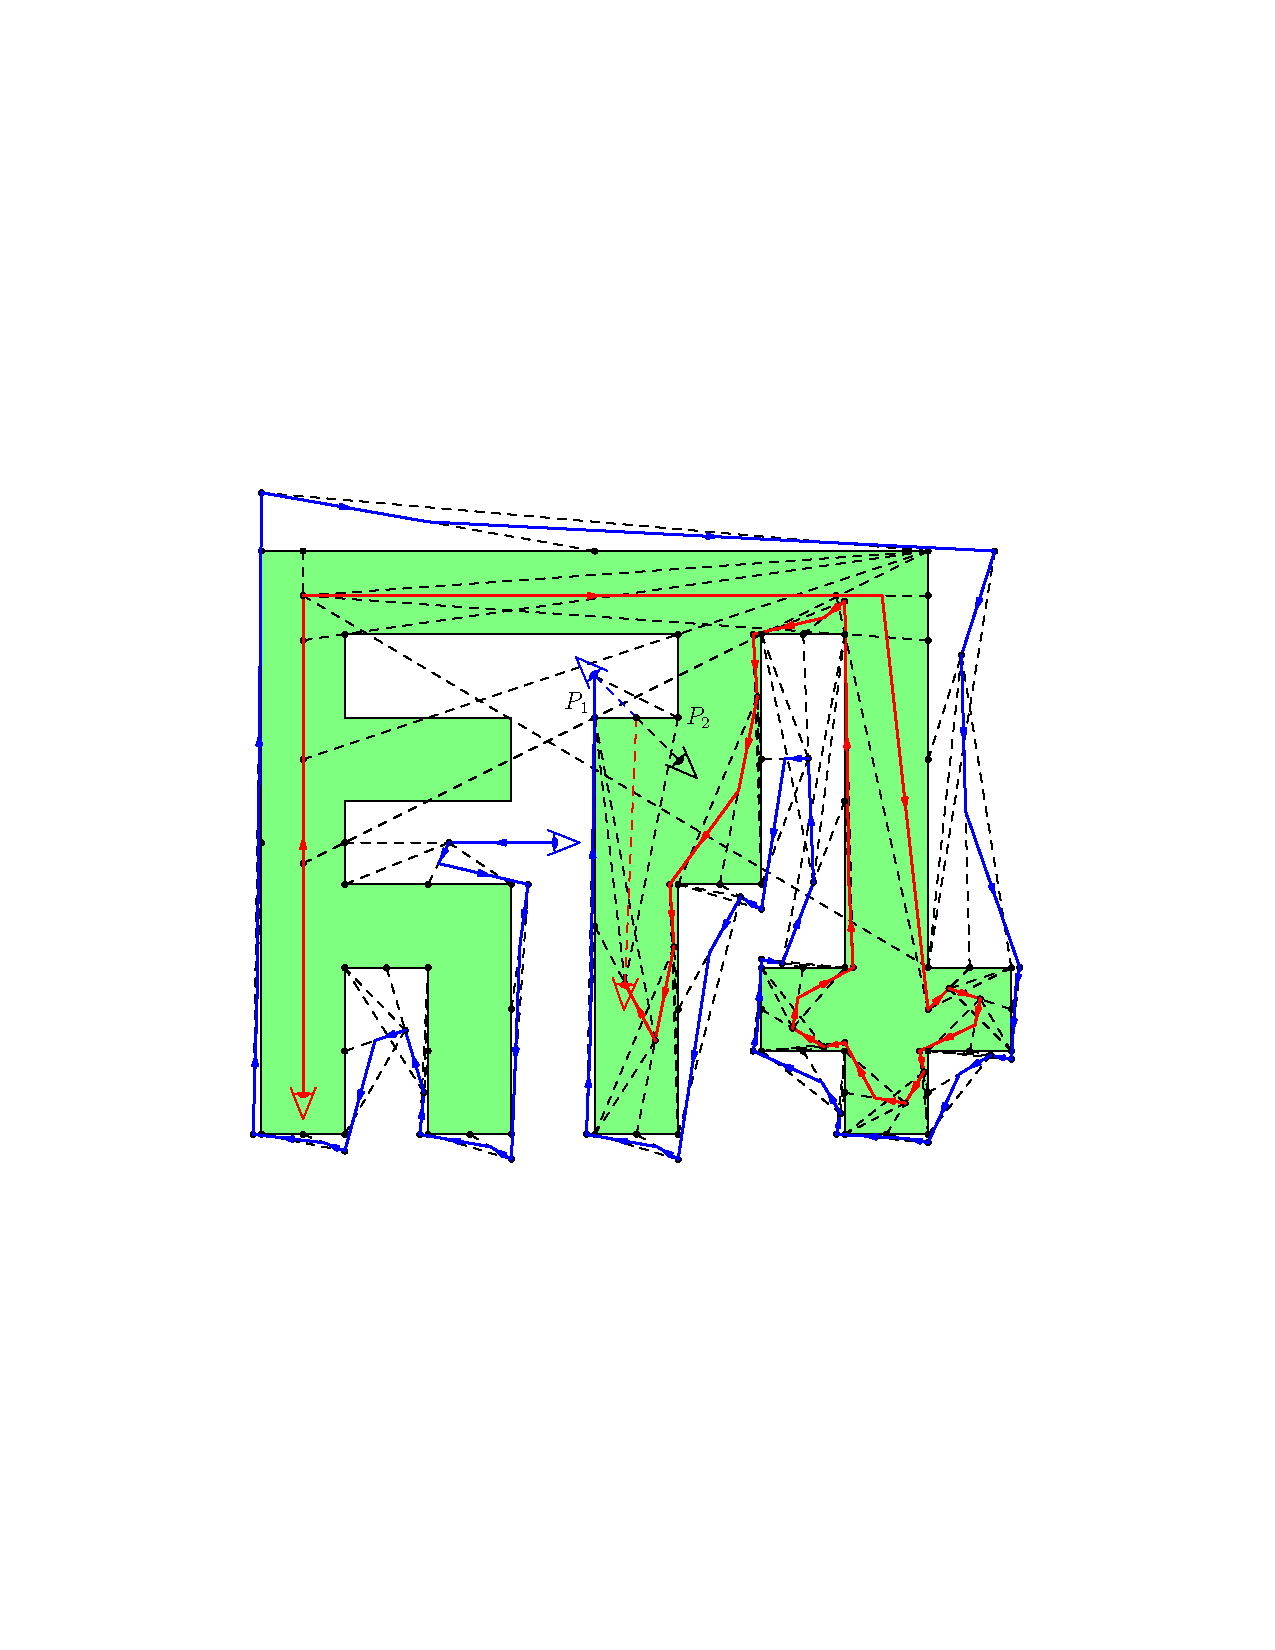
\includegraphics{jordanVerification2/SketchProofFull}
  \caption{Navigating a Maze with Theorem~\ref{eq:Squeeze2}}
  \label{fig:SketchProofJordan2Full}
\end{figure}

\section{Final Steps}
We are almost there. To finish the proof, we will need to show that when two points are on the same side of the same wall, then they are path-connected. We shall deal with this matter in \S\ref{sec:SameSideWallConnected}. First, we shall deal with the neglected matter of how we are able to obtain line-of-sight to a wall in the first place. Both problems will have us reusing our near ubiquitous Theorem~\ref{eq:Squeeze2}.

\subsection{Getting onto the Maze}
If we take an arbitrary point $X$ in the plane and an arbitrary point $X'$ on a simple polygon, then a simple ray-cast gives us line-of-sight to some other point $X''$ of the maze. If this point $X''$ lies between two other vertices, we have a line-of-sight to a wall. 

However, if $X''$ coincides with a vertex as shown in Figure~\ref{fig:SightToWall}, we will need to rotate our line-of-sight slightly. We will first assume, without loss-of-generality (or more accurately, we will assume we have rotated the polygon's vertex list) so that the vertex $X''$ coincides with the vertex $P_2$. We will want to obtain line-of-sight to either the wall $P_1P_2$ or $P_2P_3$.

\begin{figure}
  \centering\includegraphics[scale=0.75]{jordanVerification2/SightToWall}
  \caption{Obtaining Line-of-sight with a Wall}
  \label{fig:SightToWall}
\end{figure}

We can do this by applying Theorem~\ref{eq:Squeeze2} to the wall $P_1P_2$ and the polygonal fragment $P_3P_4\ldots P_n$ as described in \S\ref{sec:RotateToNew}. This will not generally give us our required point of intersection. In fact, it might be that there is \emph{no} line-of-sight from $X$ to the wall $P_1P_2$, because the wall $P_2P_3$ is in the way. 

This does not pose much of a problem. If the segment $XY$ intersects $P_3X''$ at the point $Y$, then we shall just take $Y$ as our line-of-sight. We just need two steps for this, one exploiting our linear reasoning tactic and the other our incidence discoverer, to show that the segment $XY'$ is our required line-of-sight. On the other hand, if $XY$ does not intersect $P_3X''$, then one step with our incidence reasoning tactic verifies that it is the required line-of-sight. 

We have formalised the result retaining the without-loss-of-generality assumption. This allows the reader to review which hypotheses are actually needed for this particular theorem. This is one of the great benefits of formal verification. The labour involved in teasing out the necessary hypotheses means we usually end up with very tight lemmas with which to easily trace dependencies. Consider that this theorem appears in our theory file before simple polygons are even \emph{defined}:
\begin{equation}\label{eq:RotateToWall}
  \begin{split}
  % "!P1 P2 P3 Ps X 'a.
  %  on_plane P1 'a /\ on_plane P2 'a /\ on_plane P3 'a /\ on_plane X 'a
  %  /\ (!P. MEM P Ps ==> on_plane P 'a)
  %  /\ ~between P1 P3 P2 /\ ~between P2 P1 P3
  %  /\ ~(P1 = P2) /\ ~(P1 = P3)
  %  /\ ~on_polyseg (CONS P3 Ps) P2
  %  /\ ~(?Z. between P1 Z P2 /\ on_polyseg (CONS P2 (CONS P3 Ps)) Z)
  %  /\ ~(?Z. between P2 Z P3 /\ on_polyseg (CONS P3 Ps) Z)
  %  /\ ~on_polyseg (CONS P1 (CONS P2 (CONS P3 Ps))) X
  %  /\ ~(?Z. between P2 Z X /\ on_polyseg (CONS P1 (CONS P2 (CONS P3 Ps))) Z)
  %  ==> ?Y. (between P1 Y P2 \/ between P2 Y P3)
  %          /\ ~(?Z. between X Z Y
  %                   /\ on_polyseg (CONS P1 (CONS P2 (CONS P3 Ps))) Z)"
\vdash&\neg\between{P_1}{P_3}{P_2} \wedge \neg\between{P_2}{P_1}{P_3} \wedge P_1 \neq P_2 \wedge P_1 \neq P_3\\
    &\wedge\neg\code{on\_polypath}\ (\cons{P_3}{Ps})\ P_2\\
    &\wedge(\neg\exists Z. \between{P_1}{Z}{P_2} \wedge \code{on\_polypath}\ (\cons{P_2}{\cons{P_3}{Ps}})\ Z)\\
    &\wedge(\neg\exists Z. \between{P_2}{Z}{P_3} \wedge \code{on\_polypath}\ (\cons{P_3}{Ps})\ Z)\\
    &\wedge\neg\code{on\_polyseg}\ (\cons{P_1}{\cons{P_2}{\cons{P_3}{Ps}}})\ X\\
    &\wedge(\neg\exists Z. \between{P_2}{Z}{X} \wedge \code{on\_polypath}\ (\cons{P_1}{\cons{P_2}{\cons{P_3}{Ps}}})\ Z)\\
    &\implies\exists Y. (\between{P_1}{Y}{P_2} \vee \between{P_2}{Y}{P_3})\\
    &\qquad \wedge \neg(\exists Z. \between{X}{Z}{Y} \wedge \code{on\_polypath}\ (\cons{P_1}{\cons{P_2}{\cons{P_3}{Ps}}})\ Z)
  \end{split}
\end{equation}

We can now put any point on to the maze, and thus we can connect every point in the plane to another point with line-of-sight to any wall. This means that, if we have three points in the plane, we can find three paths which bring them together at the same wall. It is enough now to verify that two of the three points are segment-connected.

\subsection{There are at most Two Regions}\label{sec:SameSideWallConnected}
Here is where we are: we have three points with line-of-sight to a wall $P_1P_2$ (without loss of generality). We know that two of these points $X$ and $Y$ are on the same side of $P_1P_2$. We will show that these two points can be path-connected.

First off, we have to consider that $X$ and $Y$ have line-of-sight to \emph{different} points $X'$ and $Y'$. Our diagrams so far in this chapter have given a different impression, but most of the points obtained in our proofs up to now ultimately rely on Axiom~\ref{eq:g22}. This axiom allows us to extend a line-segment, but there are many possible witnesses for its existential conclusion, and we have generally allowed the abstraction to proliferate in our theory, rather than eliminating it with the epsilon-operator. 

\begin{figure}
\centering\includegraphics[scale=0.6]{jordanVerification2/SameSideWallConnected1}
\caption{Connecting the Final Points}
\label{fig:SameSideWallConnected}
\end{figure}

Consider the scenario depicted in Figure~\ref{fig:SameSideWallConnected}(a). Here, our points $X$ and $Y$ have line-of-sight to different points on the same wall, so our first order of business is to get $X$ and $Y$ to have line-of-sight to the same point. Again, we use Theorem~\ref{eq:Squeeze2} against the fragment $P_2P_3\ldots P_n$, moving $X$ along its line-of-sight to a point $X''$ so that it now has line-of-sight with $Y'$. A second application of the same theorem, moving along our new line-of-sight sees us facing the point $Y$. With the two points in each other's sights, we have the last piece of our path.

We are almost home free. We still need to factor in the fact that $X$ and $Y$ are on the same side of $P_1P_2$. This is needed because we only applied Theorem~\ref{eq:Squeeze2} to the fragment $P_2P_3\ldots P_n$. The resulting lines-of-sight will not intersect this fragment, but we will need to account for the segment $P_1P_2$ separately.

Yet again, this is settled with our theorems for half-planes. Since $X$ lies on the same side of $P_1P_2$ as $Y$, and $X'$ lies on $P_1P_2$, all points on the segment $XX''$ must also lie on the same side. The same argument applies to the segment $X''Y'$, and finally to $Y'Y$. Since all of these points are on the same side of $P_1P_2$, they must lie off the line $P_1P_2$. 

The final extract of the verified proof, witnessing the final path and showing this line of argument, is reproduced in Figure~\ref{fig:SameSideWallConnectedExtract}. We have omitted references to earlier steps.

\begin{equation}
  \label{eq:SameSideWallConnected}
  \begin{split}
  % "!P1 P2 Ps X Y hand hand' hp 'a. 
  %    on_plane P1 'a /\ on_plane P2 'a
  %    /\ (!P. MEM P Ps ==> on_plane P 'a)
  %    /\ on_plane X 'a /\ on_plane Y 'a
  %    /\ between P1 hand P2 /\ between P1 hand' P2
  %    /\ ~on_polyseg (CONS P1 (CONS P2 Ps)) X
  %    /\ ~on_polyseg (CONS P1 (CONS P2 Ps)) Y
  %    /\ ~(?Z. between X Z hand /\ on_polyseg (CONS P1 (CONS P2 Ps)) Z)
  %    /\ ~(?Z. between Y Z hand' /\ on_polyseg (CONS P1 (CONS P2 Ps)) Z)
  %    /\ ~(?Z. between P1 Z P2 /\ on_polyseg (CONS P2 Ps) Z)
  %    /\ on_line P1 (line_of_half_plane hp) /\ on_line P2 (line_of_half_plane hp)
  %    /\ on_half_plane hp X /\ on_half_plane hp Y
  %    ==> seg_connected 'a (on_polyseg (CONS P1 (CONS P2 Ps))) X Y"
\vdash &\neg\code{on\_polypath}\ (\cons{P_1}{\cons{P_2}{Ps}})\ X \wedge\neg\code{on\_polypath}\ (\cons{P_1}{\cons{P_2}{Ps}})\ Y\\
    &\wedge\between{P_1}{X'}{P_2}\wedge\between{P_1}{Y'}{P_2}\\
    &\wedge\neg(\exists Z. \between{X}{Z}{X'} \wedge \code{on\_polypath}\ (\cons{P_1}{\cons{P_2}{Ps}})\ Z)\\
    &\wedge\neg(\exists Z. \between{Y}{Z}{Y'} \wedge \code{on\_polypath}\ (\cons{P_1}{\cons{P_2}{Ps}})\ Z)\\
    &\wedge\neg(\exists Z. \between{P_1}{Z}{P_2} \wedge \code{on\_polypath}\ (\cons{P_2}{Ps})\ Z)\\
    &\wedge \code{on\_line}\ P1\ \code{line\_of\_half\_plane}\ hp) \wedge \code{on\_line}\ P2\ \code{line\_of\_half\_plane}\ hp)\\
    &\wedge \code{on\_half\_plane}\ hp\ X \wedge \code{on\_half\_plane}\ hp\ Y\\
    &\implies \code{path\_connected}\ (\code{on\_polypath}\ (\cons{P_1}{\cons{P_2}{Ps}})\ X\ Y
  \end{split}
\end{equation}

\begin{boxedfigure}
\small
\begin{align*}
  % ;take ["[X:point;s:point;s':point;Y:point]"]
  % ;tactics [REWRITE_TAC [NOT_CONS_NIL;GSYM IN_SET_OF_LIST;HD;LAST
  % ;DISJOINT_IMP;set_of_list]
  % THEN REWRITE_TAC [FORALL_IN_INSERT;NOT_IN_EMPTY]]
  % ;obviously (by_planes o Di.conjuncts)
  % (thus "on_plane s 'a /\ on_plane s' 'a 
  % /\ on_plane X 'a /\ on_plane Y 'a"
  % from [0;2;3;11;12;18])
  % ;have "on_line hand (line_of_half_plane hp)
  % /\ on_line hand' (line_of_half_plane hp)"
  % from [3;8] by [g12;g21]
  % ;hence "on_half_plane hp s /\ on_half_plane hp s'
  % /\ !Z. between s Z s' \/ between s' Z Y
  % ==> on_half_plane hp Z"
  % from [8;12;16;18] by [bet_on_half_plane;bet_on_half_plane2]
  % at [20]
  % ;have "!Z. on_half_plane hp Z ==> ~on_polyseg [P1;P2] Z"
  % from [3;8] by [on_polyseg_pair;g12;g21;half_plane_not_on_line]
  % ;hence "!Z. on_polyseg [s;s';Y] Z ==> ~on_polyseg [P1;P2] Z"
  % from [8;20] by [on_polyseg_CONS2;on_polyseg_sing] at [21]
  % ;have "!Z. between s Z s' ==> ~on_polyseg (CONS P2 Ps) Z" proof
  % [fix ["Z:point"]
  % ;assume "between s Z s'"
  % ;hence "between s Z hand'" from [18]
  % using ORDER_TAC `{hand':point,s,s',Z}`
  % ;qed from [13]]
  % ;qed from [4;13;14;18;19;21] by
  % [IN;on_polyseg_CONS2;on_polyseg_sing;BET_SYM]]]];;
  &\code{take}\ [X,X'',X''',Y]\\
  &\code{have}\ \code{on\_line}\ X'\ (\code{line\_of\_half\_plane}\ hp)\\
  &\qquad\wedge \code{on\_line}\ Y'\ (\code{line\_of\_half\_plane}\ hp)\\
  &\qquad\code{from}\ \ldots\ \code{by}\ \eqref{eq:g12},\eqref{eq:g21}\\
  &\code{hence}\ \code{on\_half\_plane}\ hp\ X'' \wedge \code{on\_half\_plane}\ hp\ X'''\\
  &\qquad\wedge\forall Z. \between{X''}{Z}{X'''} \vee \between{X'''}{Z}{Y}\ \code{from} \ldots\ \code{by}\ \eqref{eq:betOnHalfPlane1},\eqref{eq:betOnHalfPlane2}\\
  &\code{have}\ \forall Z. \code{on\_half\_plane}\ hp\ Z \implies \neg\code{on\_polypath}\ [P_1,P_2]\ Z\
  \code{from}\ 3,8\\
  &\qquad\code{by}\ \eqref{eq:OnPolyPath},\eqref{eq:g12},\eqref{eq:g21},\eqref{eq:halfPlaneNotOnLine}\\
  &\code{hence}\ \forall Z. \code{on\_polypath}\ [X'',X'',Y]\ Z \implies \neg\code{on\_polypath}\ [P_1,P_2]\ Z\\
  &\qquad\code{from} \ldots\ \code{by}\ \eqref{eq:OnPolyPath}\ & 21\\
  &\code{have}\ \forall Z. \between{X''}{Z}{X'''} \implies \neg\code{on\_polypath}\ (\cons{P_2}{Ps})\ Z\ \code{proof}\\
  &\qquad \code{fix}\ Z\\
  &\qquad \code{assume}\ \between{X''}{Z}{X'''}\\
  &\qquad \code{hence}\ \between{X''}{Z}{Y'}\ \code{from}\ \ldots\ \code{using}\ \code{ORDER\_TAC}\ \{X'',X''',Y',Z\}\\
  &\qquad \code{qed}\ \code{from}\ \ldots\\
  &\code{qed}\ \code{from}\ \ldots,21\ \code{by}\ \eqref{eq:OnPolyPath},\eqref{eq:g21}
\end{align*}
\caption{Verification Extract for Theorem~\ref{eq:SameSideWallConnected}}
\label{fig:SameSideWallConnectedExtract}
\end{boxedfigure}

One final remark: in our sketch proof from \S\ref{sec:JordanCurveFirstProof}, we actually assumed we could carry out this argument when establishing IH3 and IH5. Once again, we are making progress towards a verification of our first point-in-polygon proof. It is interesting to realise that, even if the two proofs are conceptually very different, many of the same arguments are needed for both.

\section{Conclusion}
The proof of the final theorem puts all of the pieces together. We start from three arbitrary points in the plane not on the polygonal segment, have each obtain a line-of-sight to a wall of the maze, and then use polygon rotations and Theorem~\ref{eq:PolygonMove} to find three paths to three points with line-of-sight to the first wall of the maze. We then apply  Theorem~\ref{eq:HalfPlaneCover} which says that two of these points must be on the same side of the first wall, and thus, from Theorem~\ref{eq:SameSideWallConnected}, we know that that these two points are path-connected.

As with the final theorem in the last chapter, the final theorem here is much more readable than the lemmas considered up to now. The theory so far builds theorems with large numbers of complicated hypotheses, such as those for Theorem~\ref{eq:SameSideWallConnected} (and remember that we have not even bothered to mention all the planar hypotheses needed for every one of these theorems). When developing a theory such as this, where theorems are almost made opaque by their hypotheses, we have to pay particularly close attention to be confident that we are making progress. It was some relief when the development paid off.

\begin{align*}
\vdash &\code{simple\_polygon}\ Ps\\
       &\wedge \neg\code{on\_polyseg}\ Ps\ P\wedge \neg\code{on\_polyseg}\ Ps\ Q\wedge \neg\code{on\_polyseg}\ Ps\ R\\
       &\implies \code{seg\_connected}\ (\code{on\_polyseg}\ Ps)\ P\ Q\\
       &\qquad\quad\vee \code{seg\_connected}\ (\code{on\_polyseg}\ Ps)\ P\ R\\
       &\qquad\quad\vee \code{seg\_connected}\ (\code{on\_polyseg}\ Ps)\ Q\ R
\end{align*}

To end this chapter, we provide the diagram in Figure~\ref{fig:JordanTheoryOutline} showing the major dependencies needed to prove both parts of the Polygonal Jordan Curve Theorem. Individual boxes show the major hurdles in the theory, with their size roughly correlated with the size of the proofs needed to overcome that particular hurdle. 

\begin{figure}
\includegraphics[scale=0.5]{jordanVerification2/development}
\caption{The Theory of Polygons}
\label{fig:JordanTheoryOutline}
\end{figure}

Of the 11000 lines of code needed for the whole project, our theory of polygons comes to a modest 5000 lines of mostly synthetic proof (there are far fewer actual proof \emph{steps}). We do not believe this would have been achievable had we not had the support of our incidence discoverer, which justified 111 of our proof steps. 

As Hilbert and Veblen suggested, the theory of half-planes is crucial to the proof of the Polygonal Jordan Curve Theorem, relieving us of the burden of applying Pasch's Axiom \eqref{eq:g24}. In fact, this axiom was needed on only 11 occasions. But besides the theory of half-planes, linear ordering also had pride of place. Our automated linear reasoning tactic was used an impressive 82 times. 

We hope that our formal development contributes an interesting take on the Polygonal Jordan Curve Theorem. Our analysis has had to be far finer than that considered by either Veblen or Feigl, and thus we have introduced some new ideas to understand the mechanics of the proof. In particular, we would like to believe that the use of intuitive metaphors such as ``lines-of-sight'' in this chapter has kept things lively and geometrically focused, and made the details of our proofs all the more clear. 

Most importantly, though, as is the case with all formal verification projects, we have forever set the validity of the mathematical arguments in these chapters beyond reproach. The question of whether the Polygonal Jordan Curve Theorem is a theorem of ordered geometry is now settled definitively even to the most \emph{hardened} sceptic, who in this case, has taken the guise of an extremely pedantic computer system: HOL~Light.

%%% Local Variables: 
%%% TeX-master: "../thesis"
%%% End: 
